
\documentclass{article}
\usepackage[T1]{fontenc}\usepackage[utf8]{inputenc}
\usepackage{lmodern}
\usepackage{graphicx}
\usepackage{textcomp}
\usepackage{lastpage}
\usepackage[section]{placeins}
\usepackage[hidelinks]{hyperref}
\usepackage{fancyhdr}
\usepackage{nameref}

\makeatletter
\newcommand*{\currentname}{\@currentlabelname}
\makeatother

\begin{document}

\pagestyle{fancy}
\fancyhf{}
\fancyhead[L]{Page ends at \currentname}
\fancyfoot[C]{Page \thepage}
\renewcommand{\headrulewidth}{1pt}

\renewcommand*\contentsname{Table of Contents}
\tableofcontents
\renewcommand{\listfigurename}{Illustrations}
\listoffigures
\newpage

\section{Firewall Rules}
\label{sec:Firewall RulesID}

	\FloatBarrier
	\subsection{Affected interface}
	\label{subsec:Affected interfaceID}

	We then modify the previous homeworks' firewall rules to allow Ping, HTTP, HTTPS, and DNS for ServerNet from WAN not LAN, rules are shown in figure 1.

		\FloatBarrier
		\begin{figure}[h!]
			\centering
			\frame{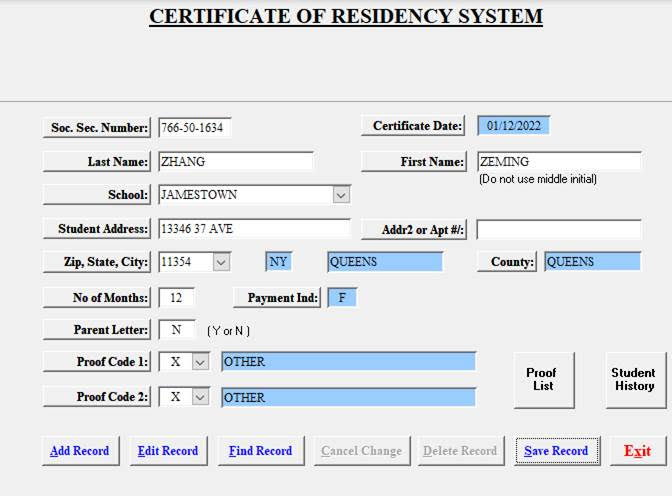
\includegraphics[width=0.75\textwidth]{figure1.png}}
			\caption{Screenshot of firewall rules to allow one device}
		\end{figure}
		\FloatBarrier


	We then access pfsense through the ServerGUI as we assign that to be the only device to connect to pfsense. We will find the protocol and ports used by HTTP(s), Ping and DNS to implement rules that allow only the ServerNet interface to do Ping etc. The rules are shown in figure 2.

		\FloatBarrier
		\begin{figure}[h!]
			\centering
			\frame{
\includegraphics[width=0.75\textwidth]{figure2.png}}
			\caption{Screenshot of firewall rules to allow Ping, HTTP, HTTPS, and DNS}
		\end{figure}
		\FloatBarrier


\section{Linux Server Setup}
\label{sec:Linux Server SetupID}

	\FloatBarrier
	\subsection{Initial installation details}
	\label{subsec:Initial installation detailsID}

	After finding the iso in drive 1, ISO directory, Linux subdirectory with information we power on the system and began setup.

		\FloatBarrier
		\begin{figure}[h!]
			\centering
			\frame{
\includegraphics[width=0.75\textwidth]{figure3.png}}
			\caption{Screenshot of Ubantu Server lang Options}
		\end{figure}
		\FloatBarrier


	The figure below are keyboard language options. Just stick with english.

		\FloatBarrier
		\begin{figure}[h!]
			\centering
			\frame{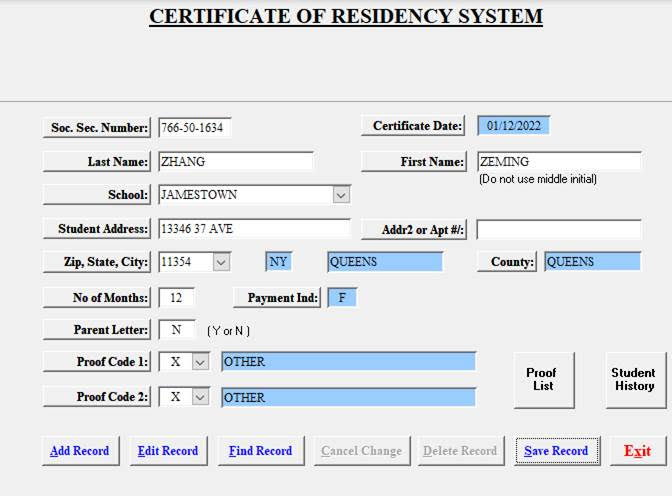
\includegraphics[width=0.75\textwidth]{figure4.png}}
			\caption{Screenshot of Ubantu Server keyboard lang Options}
		\end{figure}
		\FloatBarrier


	This is the network setup, just go with default.

		\FloatBarrier
		\begin{figure}[h!]
			\centering
			\frame{
\includegraphics[width=0.75\textwidth]{figure5.png}}
			\caption{Screenshot of Ubantu Server network Options}
		\end{figure}
		\FloatBarrier


	This is the storage setup, just go with default and click done.

		\FloatBarrier
		\begin{figure}[h!]
			\centering
			\frame{
\includegraphics[width=0.75\textwidth]{figure6.png}}
			\caption{Screenshot of Ubantu Server storage config}
		\end{figure}
		\FloatBarrier


	We are going to set up our profile with “Server name: web28. Your name: sysadmin; username: sysadmin; password: Change.me!” we will come to an interface for language options.

		\FloatBarrier
		\begin{figure}[h!]
			\centering
			\frame{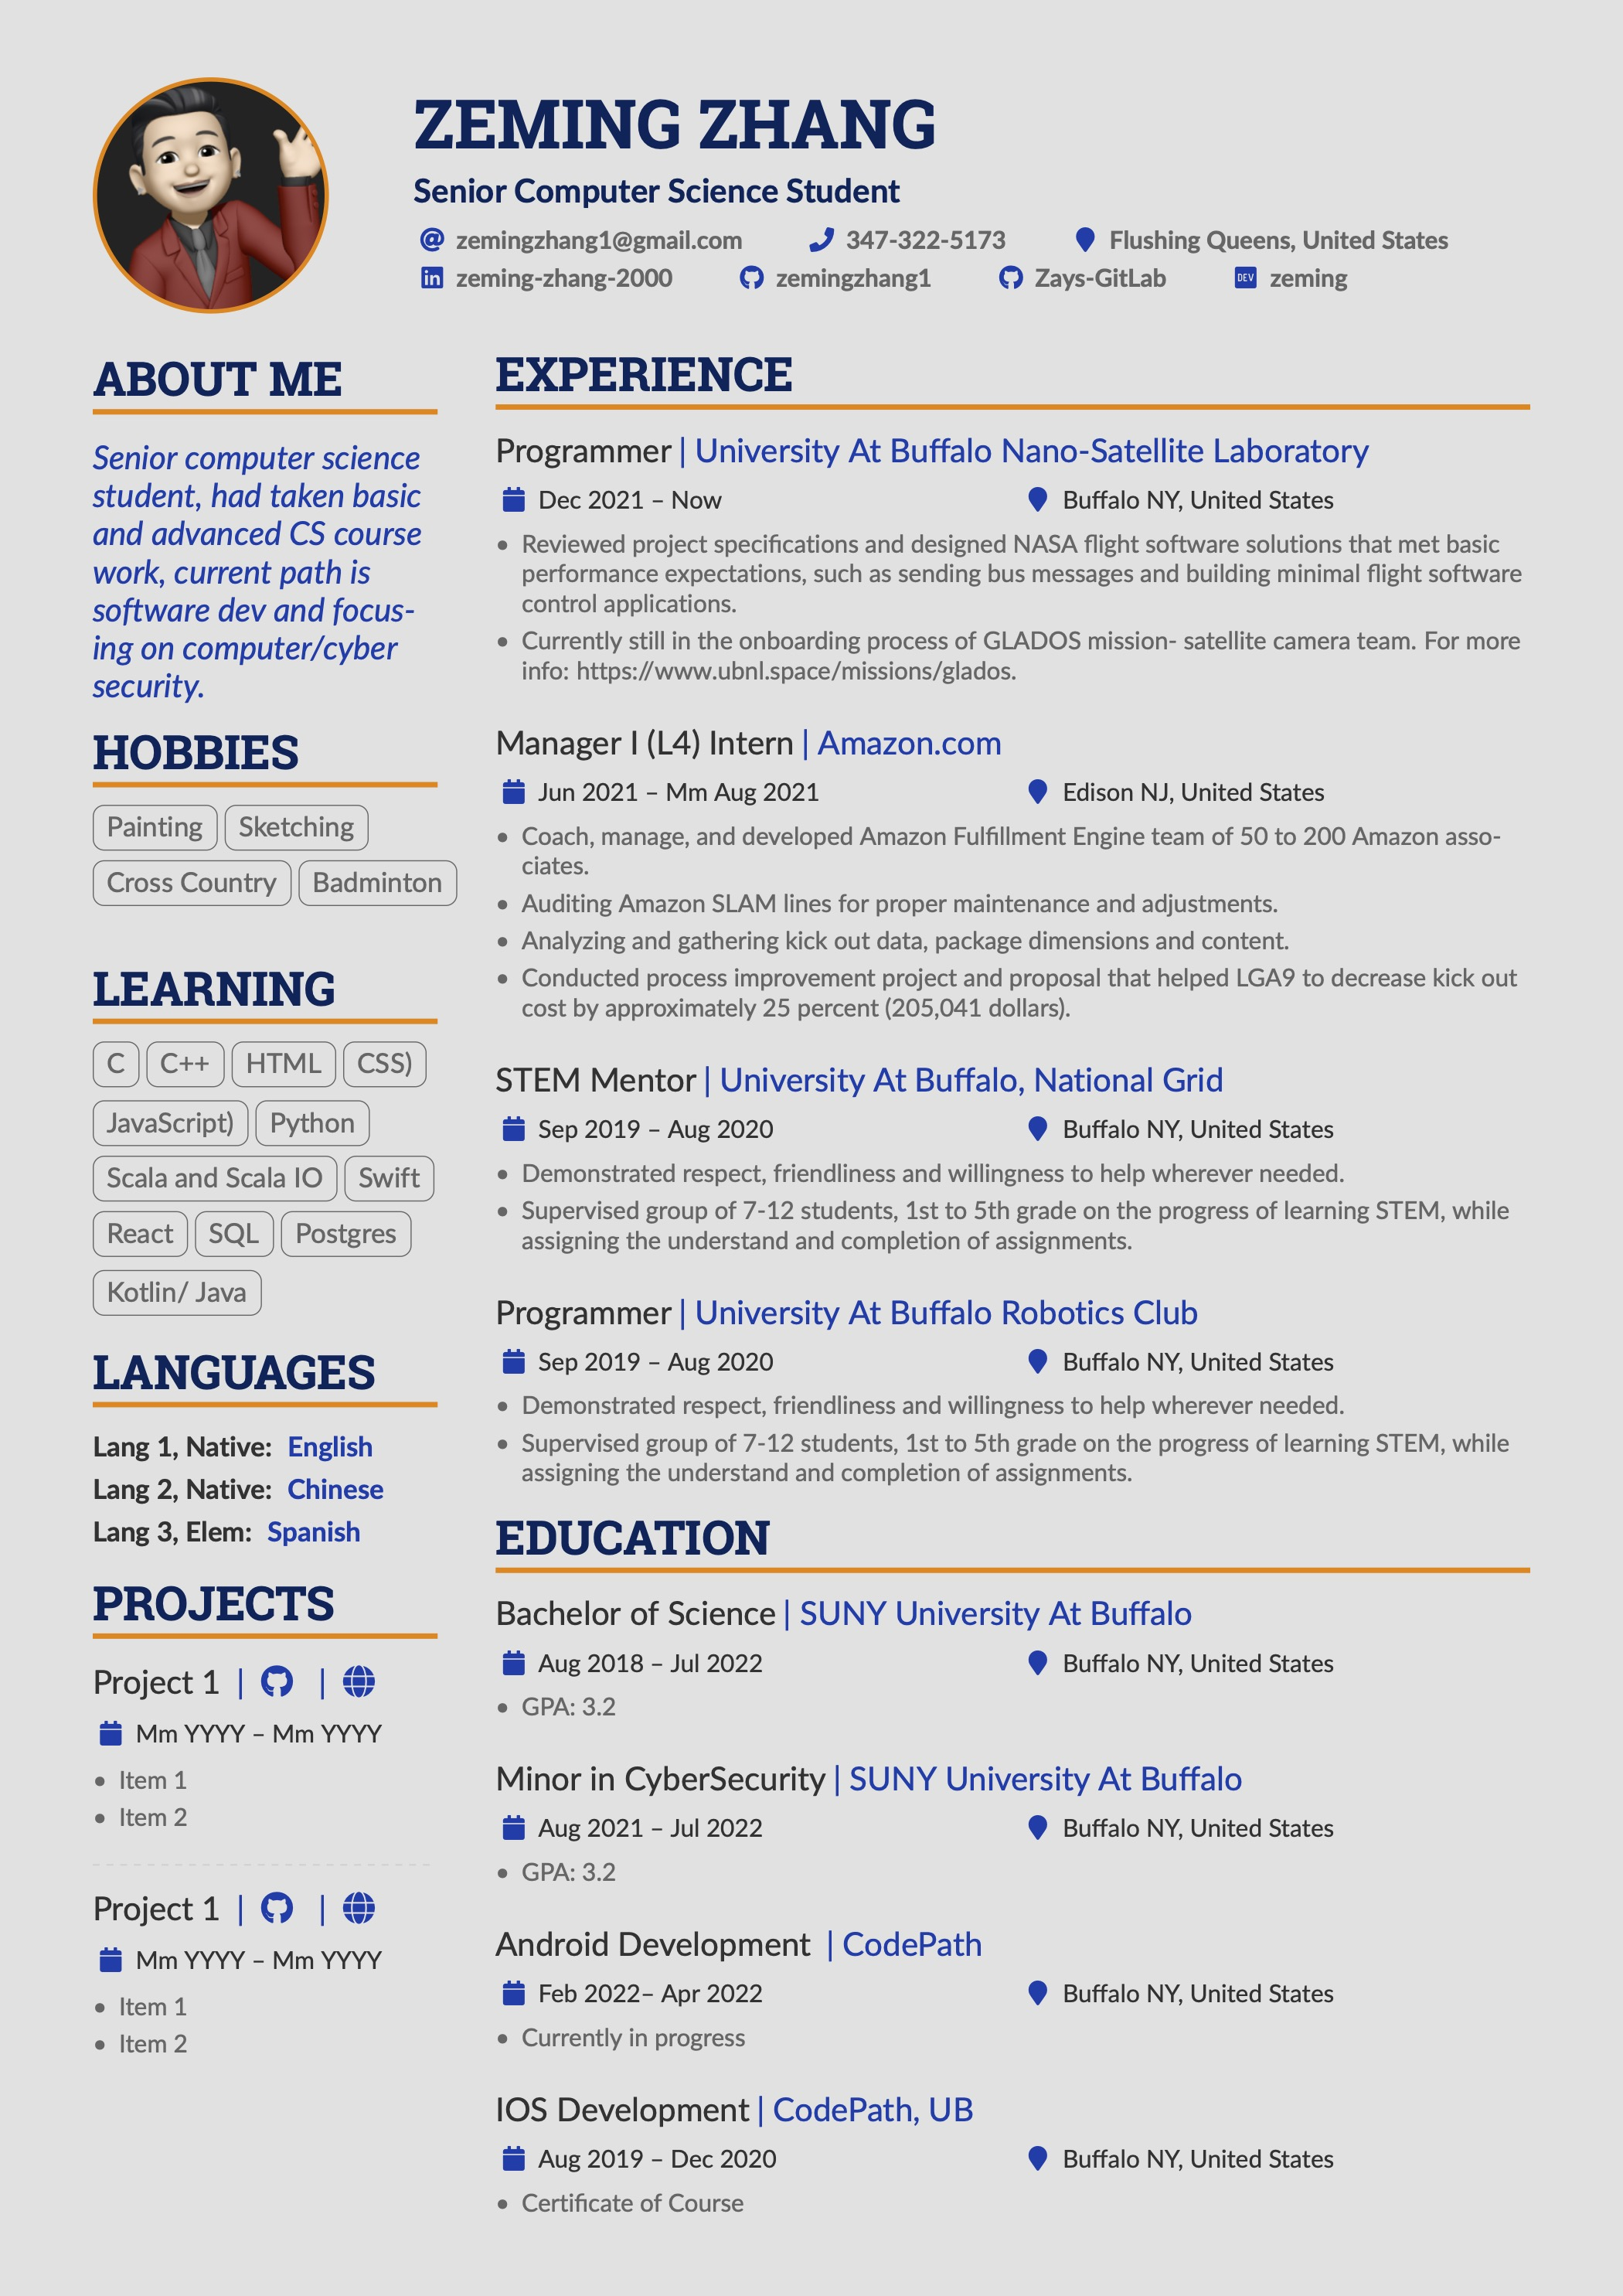
\includegraphics[width=0.75\textwidth]{figure7.png}}
			\caption{Screenshot of Ubantu Server profile setup}
		\end{figure}
		\FloatBarrier


	Good, now we can reboot it.

		\FloatBarrier
		\begin{figure}[h!]
			\centering
			\frame{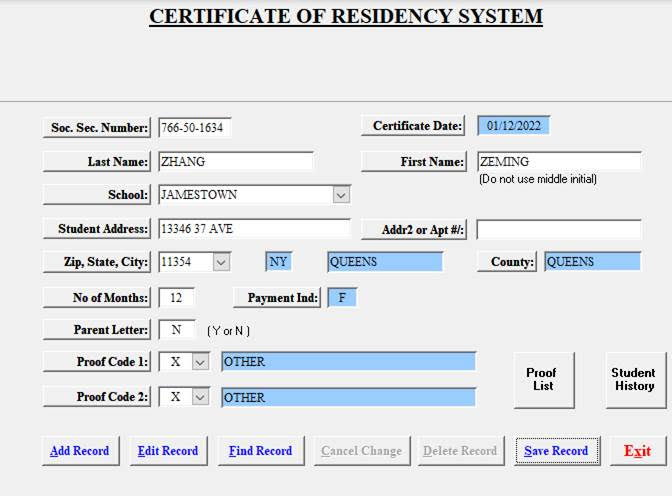
\includegraphics[width=0.75\textwidth]{figure8.png}}
			\caption{Screenshot of Ubantu Server installation complete}
		\end{figure}
		\FloatBarrier


	Relogin with the credential that was just set.

		\FloatBarrier
		\begin{figure}[h!]
			\centering
			\frame{
\includegraphics[width=0.75\textwidth]{figure9.png}}
			\caption{Screenshot of Ubantu Server reboot and login}
		\end{figure}
		\FloatBarrier


	\FloatBarrier
	\subsection{Test/verify network connectivity}
	\label{subsec:Test/verify network connectivityID}

	We will run the ip a command after changing the IP and DNS.

		\FloatBarrier
		\begin{figure}[h!]
			\centering
			\frame{
\includegraphics[width=0.75\textwidth]{figure10.png}}
			\caption{Screenshot of Ubantu Server ip a cmd}
		\end{figure}
		\FloatBarrier


	\FloatBarrier
	\subsection{OS and virtualization support software installation}
	\label{subsec:OS and virtualization support software installationID}

	We now use apt - sudo apt update and upgrade to update our OS.

		\FloatBarrier
		\begin{figure}[h!]
			\centering
			\frame{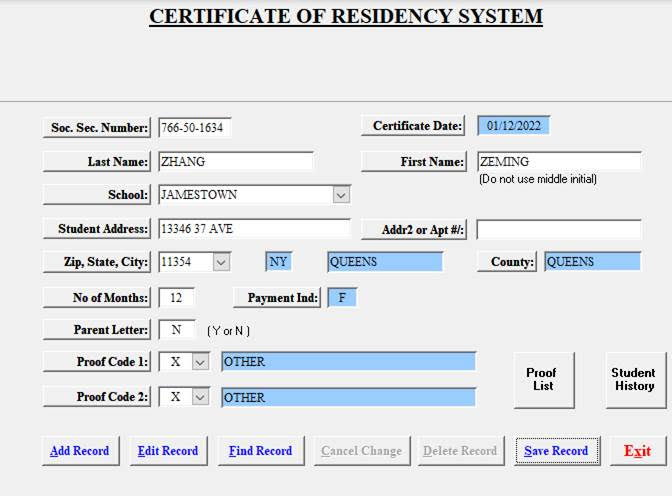
\includegraphics[width=0.75\textwidth]{figure11.png}}
			\caption{Screenshot of Ubantu server update}
		\end{figure}
		\FloatBarrier


	\FloatBarrier
	\subsection{Install additional software packages}
	\label{subsec:Install additional software packagesID}

	

\section{Install and Configure the RockyDBServer VM}
\label{sec:Install and Configure the RockyDBServer VMID}

	\FloatBarrier
	\subsection{Install/Config the RockyDBServer VM}
	\label{subsec:Install/Config the RockyDBServer VMID}

	After finding the iso in drive 1, ISO directory, Linux subdirectory with information we power on the system and began setup.

		\FloatBarrier
		\begin{figure}[h!]
			\centering
			\frame{
\includegraphics[width=0.75\textwidth]{figure12.png}}
			\caption{Screenshot of Ubantu Server lang Options}
		\end{figure}
		\FloatBarrier


	This is the Rocky installation summary interface, just go setup root and install destination.

		\FloatBarrier
		\begin{figure}[h!]
			\centering
			\frame{
\includegraphics[width=0.75\textwidth]{figure13.png}}
			\caption{Screenshot of Rocky installation summary interface.}
		\end{figure}
		\FloatBarrier


	We will set the root password to “Change.me!”.

		\FloatBarrier
		\begin{figure}[h!]
			\centering
			\frame{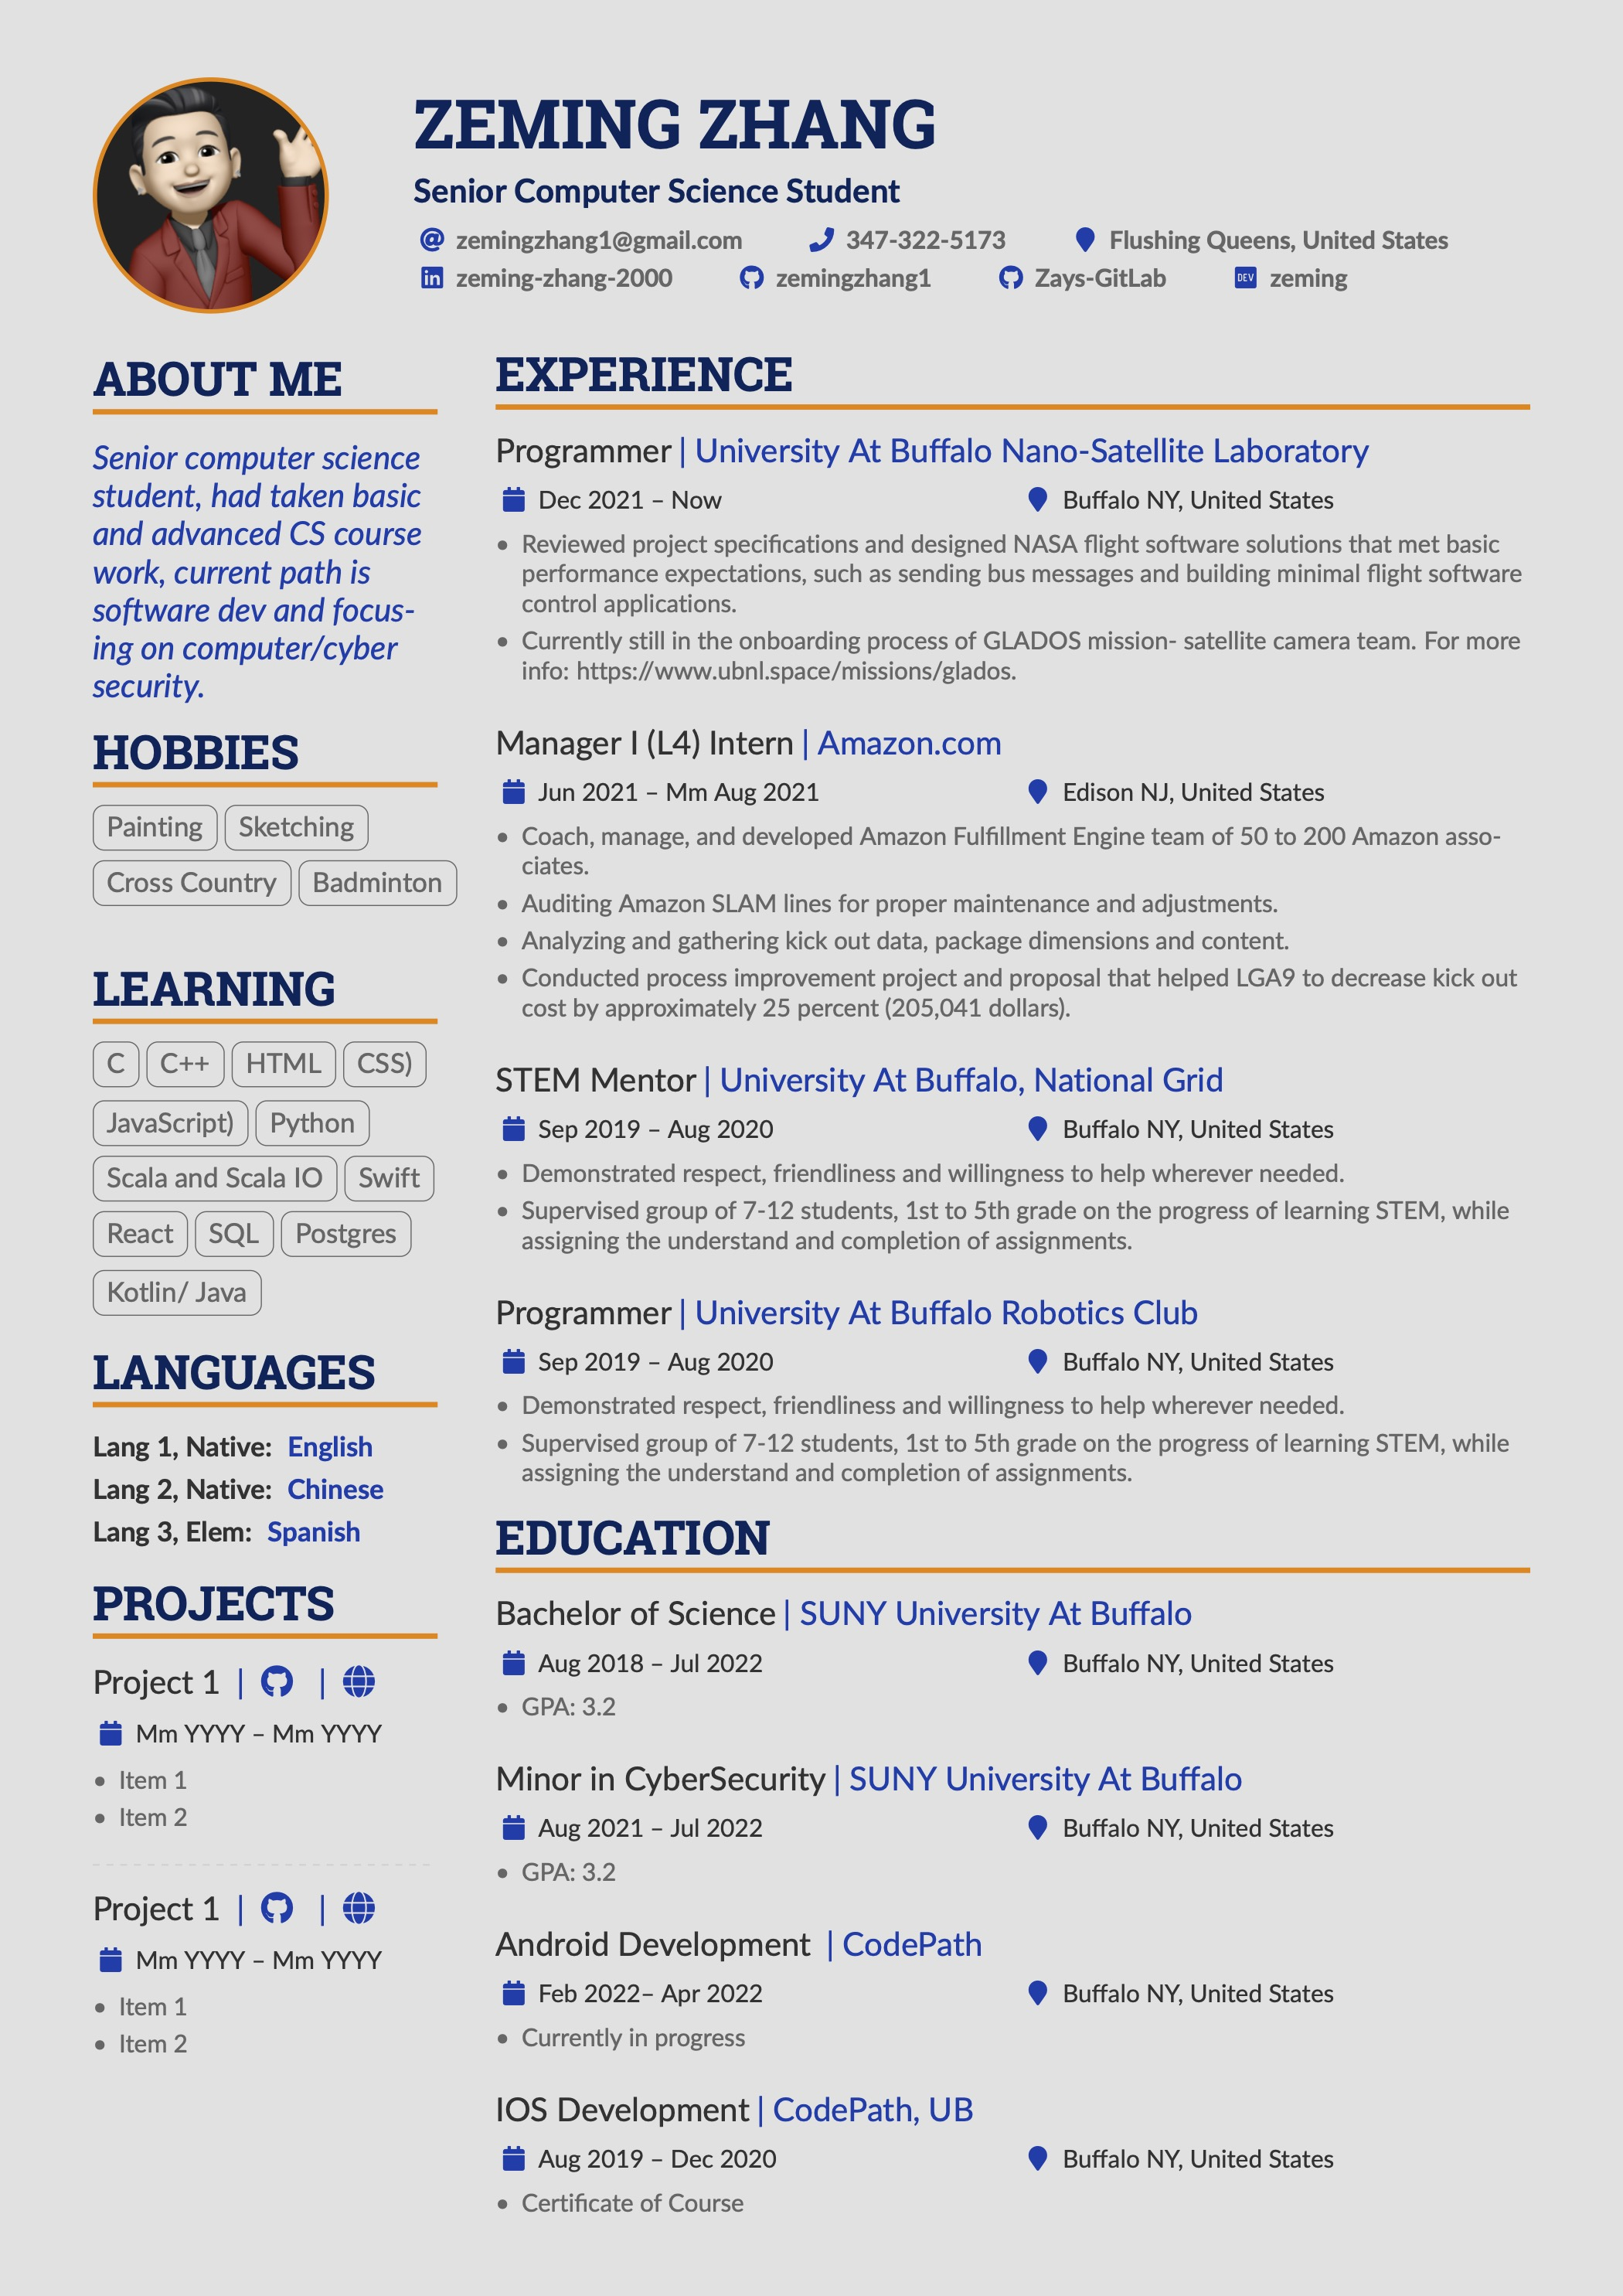
\includegraphics[width=0.75\textwidth]{figure14.png}}
			\caption{Screenshot of Rocky root password}
		\end{figure}
		\FloatBarrier


	We will then configure our storage disk destination of the file from installation.

		\FloatBarrier
		\begin{figure}[h!]
			\centering
			\frame{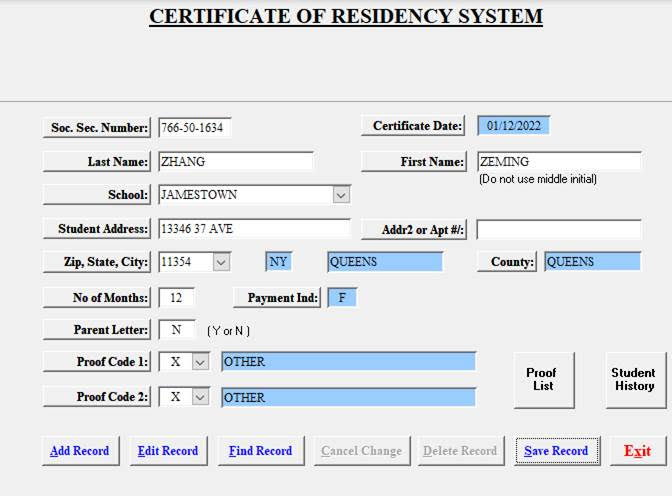
\includegraphics[width=0.75\textwidth]{figure15.png}}
			\caption{Screenshot of Rocky installment destination}
		\end{figure}
		\FloatBarrier


	We are going to set up our profile with “Full name: sysadmin; username: sysadmin; password: Change.me!”.

		\FloatBarrier
		\begin{figure}[h!]
			\centering
			\frame{
\includegraphics[width=0.75\textwidth]{figure16.png}}
			\caption{Screenshot of Rocky user creation}
		\end{figure}
		\FloatBarrier


	After we setup eventing and our credentials click done.

		\FloatBarrier
		\begin{figure}[h!]
			\centering
			\frame{
\includegraphics[width=0.75\textwidth]{figure17.png}}
			\caption{Screenshot of Rocky user credentials}
		\end{figure}
		\FloatBarrier


	Relogin with the credential that was just set.

		\FloatBarrier
		\begin{figure}[h!]
			\centering
			\frame{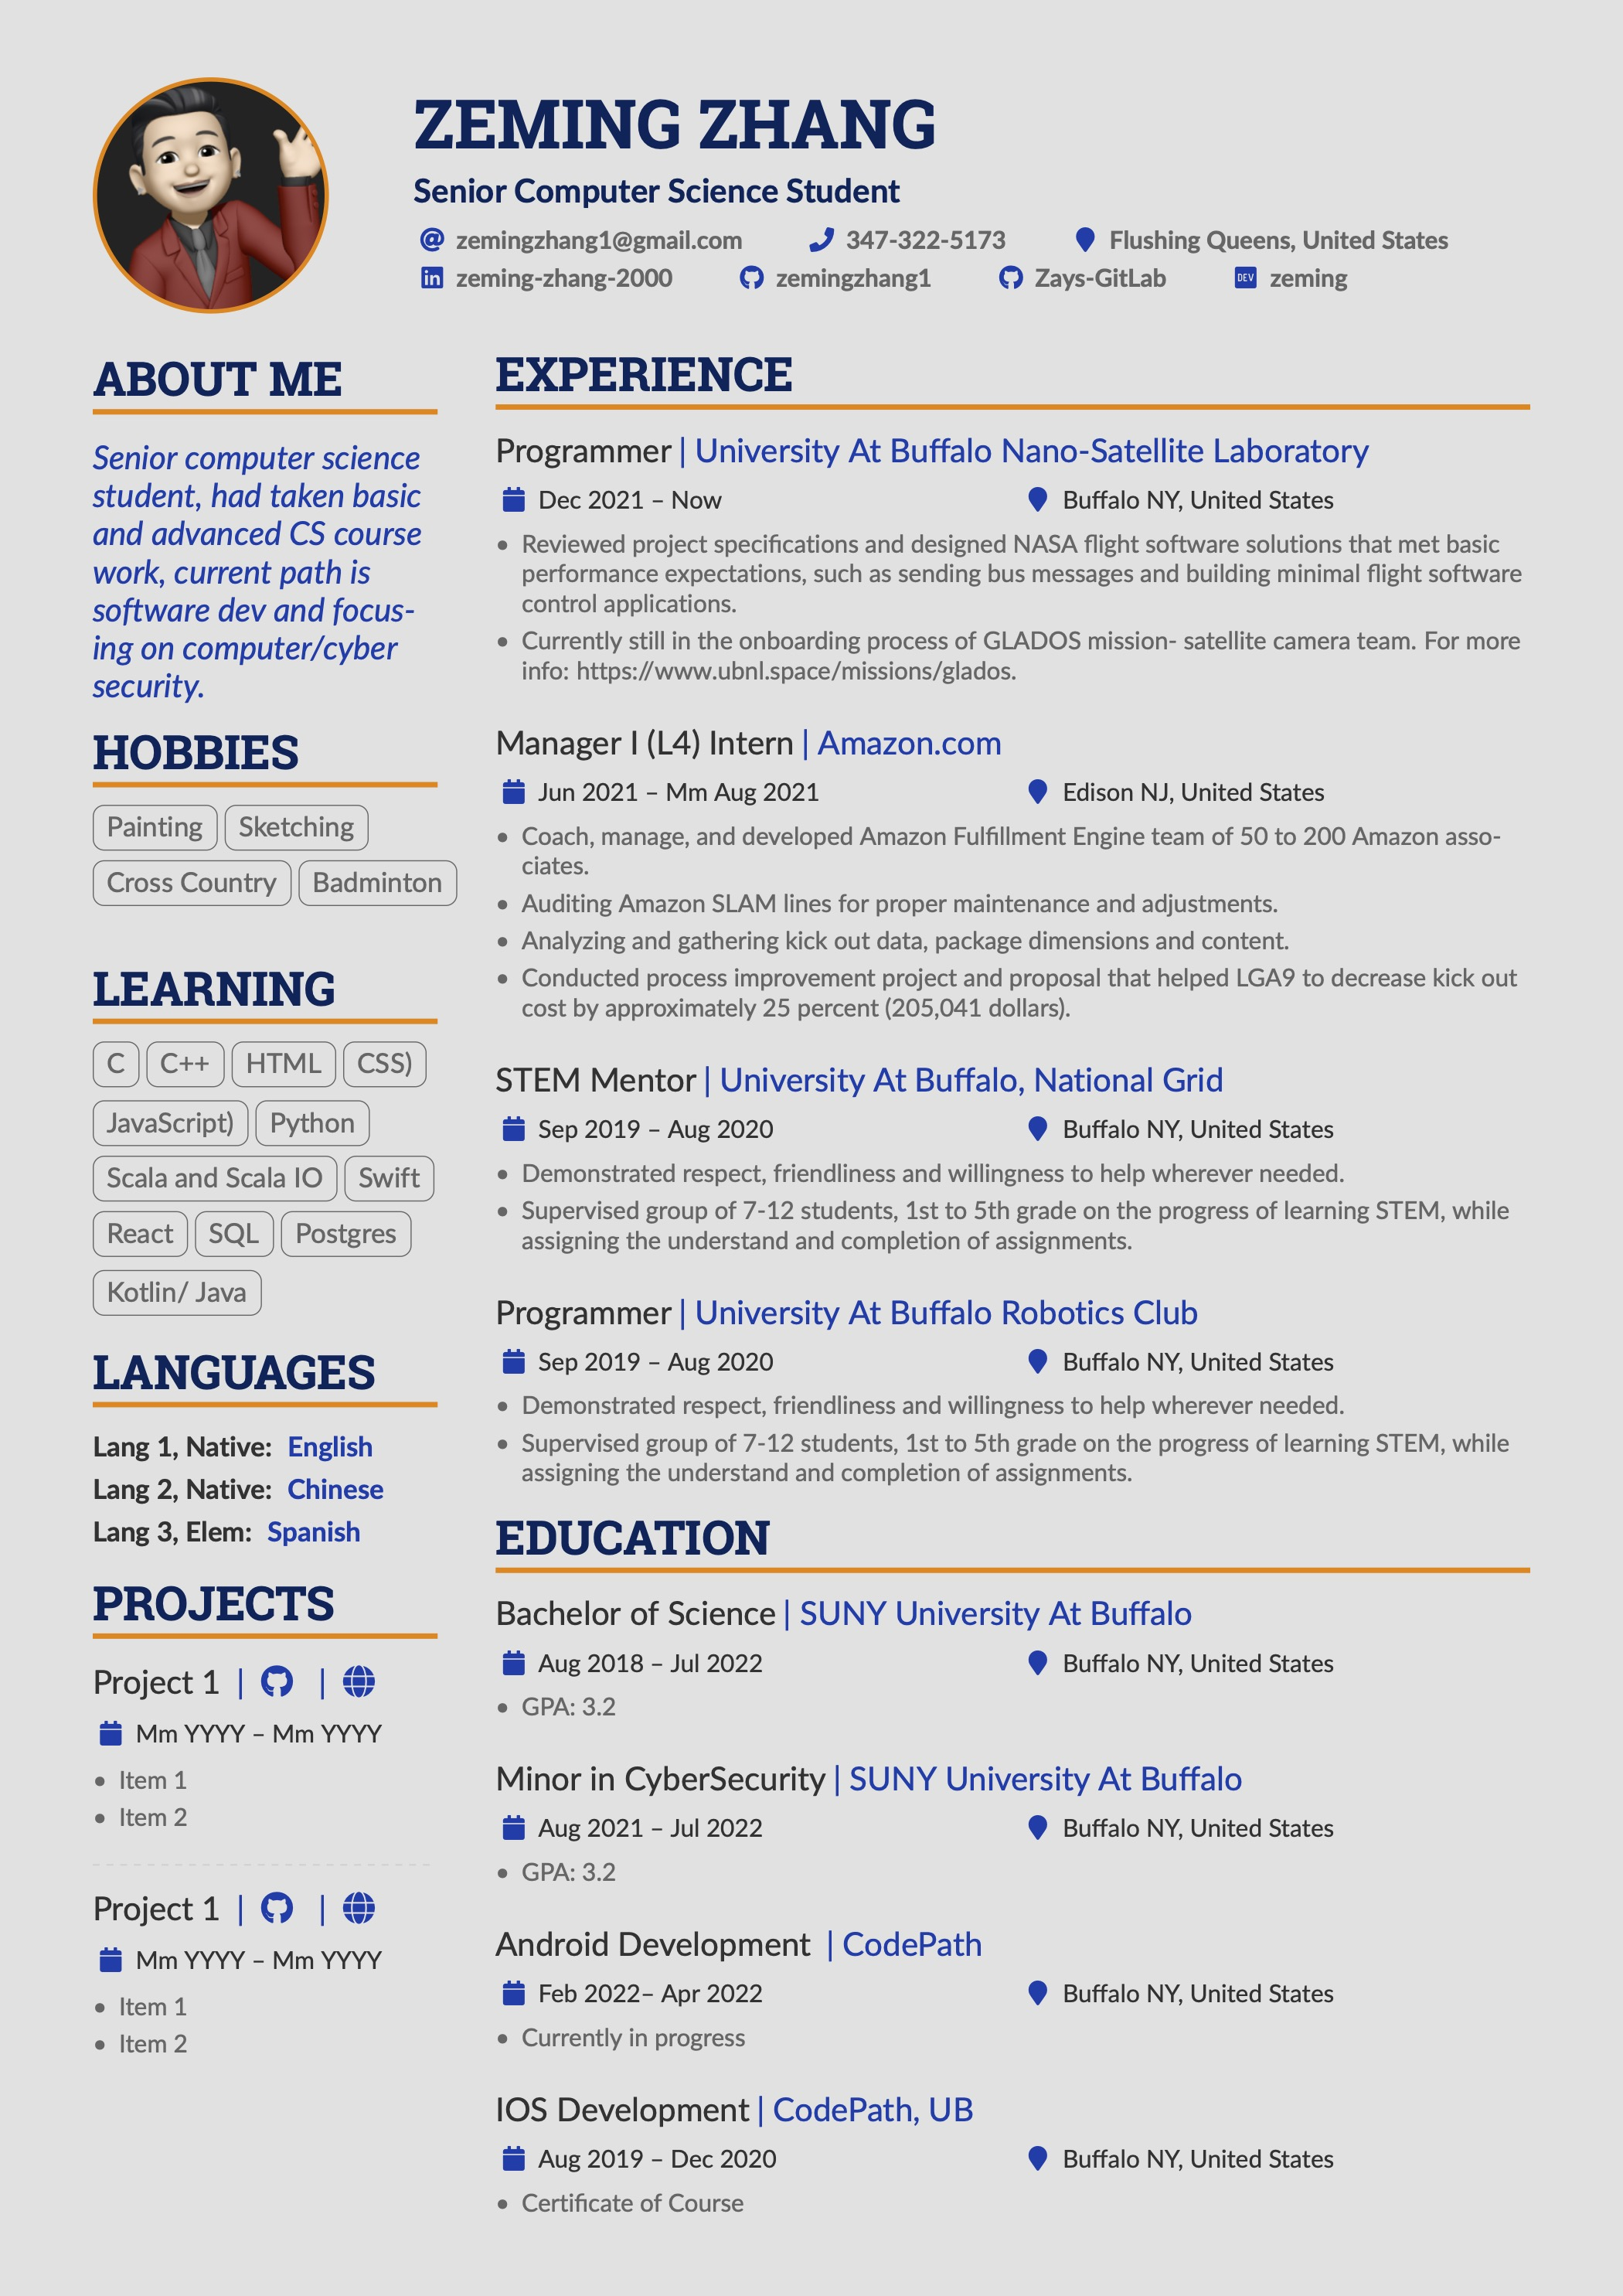
\includegraphics[width=0.75\textwidth]{figure18.png}}
			\caption{Screenshot of Rocky installment done}
		\end{figure}
		\FloatBarrier


	Re Login now to test out if it worked.

		\FloatBarrier
		\begin{figure}[h!]
			\centering
			\frame{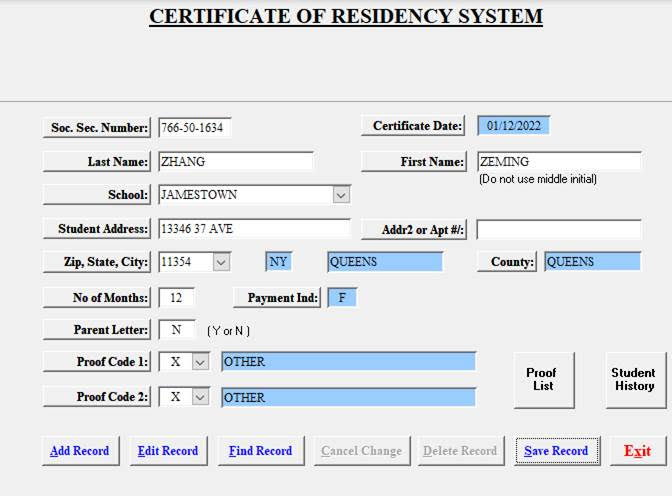
\includegraphics[width=0.75\textwidth]{figure19.png}}
			\caption{Screenshot of Rocky terminal}
		\end{figure}
		\FloatBarrier


	\FloatBarrier
	\subsection{Test/verify network connectivity}
	\label{subsec:Test/verify network connectivityID}

	

		\FloatBarrier
		\begin{figure}[h!]
			\centering
			\frame{
\includegraphics[width=0.75\textwidth]{figure20.png}}
			\caption{Screenshot of Rocky change IP}
		\end{figure}
		\FloatBarrier


	

		\FloatBarrier
		\begin{figure}[h!]
			\centering
			\frame{
\includegraphics[width=0.75\textwidth]{figure21.png}}
			\caption{Screenshot of Rocky change IP ens160}
		\end{figure}
		\FloatBarrier


	\FloatBarrier
	\subsection{OS and virtualization support software installation}
	\label{subsec:OS and virtualization support software installationID}

	

	\FloatBarrier
	\subsection{Install additional software packages}
	\label{subsec:Install additional software packagesID}

	

\section{User and Group Creation}
\label{sec:User and Group CreationID}

	\FloatBarrier
	\subsection{On UbuntuClient user and group creation}
	\label{subsec:On UbuntuClient user and group creationID}

	Contrary to popular belief, Lorem Ipsum is not simply random text. It has rootsin a piece of classical Latin literature from 45 BC, making it over 2000 years old.

\section{Linux Hardening}
\label{sec:Linux HardeningID}

	\FloatBarrier
	\subsection{Linux hardening techniques into practice}
	\label{subsec:Linux hardening techniques into practiceID}

	

\section{Update Topology}
\label{sec:Update TopologyID}

\end{document}
